\chapter{Change in English today}\label{englishtoday}
\largerpage
\section{History and context}
\subsection{What is English?}\label{what}
In the previous chapter, we saw that variation is ubiquitous. We also noted that it's the prerequisite for language change, although we didn't elaborate. Let's elaborate a little bit now: there can't be language change without there being language variation first. Throughout its history, English has changed considerably, and it has certainly been changing in the last two centuries as well. Before we plunge into the discussion of the changes affecting English recently, we need to answer two questions. What do we mean by English \textit{today}? And what do we mean by English?

The answers to the first question may vary depending on who you ask, but for our purposes we will define the English of today, or Present Day English (PDE), as starting in 1945 and continuing until, well, today! Why 1945 and not, say 1988, or 2000? The main reason is our decision to follow the time division proposed by \citet{Beal2004} for Late(r) Modern English (see \chapref{LModE}), which she defines as ending in 1945. Our decision is therefore to a large extent a conventional one. But whether we pick 1945 or 1988, from the point of view of the structure of the language in the 20th and the 21st centuries, does not make that much of a difference. But choose a starting point of some sort we must, for practical reasons, and we choose 1945, the end of the Second World War.

The other question is, however, perhaps unexpectedly, trickier -- how do we define English? What is English? This can be answered in a very wide range of ways. Some of us may think of standard English\is{standardization} -- but then there is no one standard global English;\is{globalization} instead, there are several local standards (such as Standard Southern British English,\il{English, Standard} Singapore English,\il{English, Singapore} Scottish Standard English,\il{English, Scottish} General American,\il{English, American} etc.). Furthermore, restricting ourselves to standard varieties of English would be unsatisfactory -- most speakers of English (including most non-native speakers of English) don't speak a standard variety of English, and those who do arguably do not do so all the time. Does that mean they don't speak English? Of course not. They just speak a variety other than those that happened to end up being the ones officially recognized as standard. And should we only include L1 standard and non-standard varieties of English in what we mean when we say the English language? As Míša was writing this chapter, she was writing it in (more or less) standard English, but English is not her mother tongue. Would we therefore conclude this chapter is not written in English? Of course not. There are now more non-native than native speakers of English, who use English for a variety of purposes: when travelling, in education, for entertainment, etc. \citep[68]{Crystal2003b}. Both standard and non-standard\is{standardization} varieties are part of English, and so are both native and non-native varieties. As a result, it's possible to find astoundingly diverse examples of English, but fairly often, we can also find a lot of homogeneity (or similarity) across the globe. Have a look for yourself:

\begin{itemize}
    \item But here, ja, I can get a job, but there are too much challenges. It's like, I don't know maybe if it's the area I'm staying or is it around, or is — it's about South Africa.\\	
    (Zimbabwe English;\il{English, Zimbabwe} from IDEA\footnote{\url{https://www.dialectsarchive.com/zimbabwe-6}.})
    \item Yeah, I'm gonna take my horse to the old town road. I'm gonna ride `til I can't no more. (...) I been in the valley. You ain't\is{\emph{ain't}} been up off the porch, now. Can't nobody tell me nothing. You can't tell me nothing.\\(American English,\il{English, American} \iai{Lil Nas X}, \emph{Old Town Road})
    \item I will repair tomorrow.\\(Mongolian English;\il{English, Mongolian} \citealp[215]{Cohen2005})
    \item I like very much. I been out from Miami three times. I been Orlando, and, ah, I been `94 in San Francisco to a wor, a World Cup. And most of my time is spent in Miami and, and around Miami. My hobbies is, I play soccer, ah, tennis and go to the beach, listen nice music, eat good food and meet nice girls.\\(Brazilian English;\il{English, Brazilian} from IDEA\footnote{\url{https://www.dialectsarchive.com/brazil-4}.})
    \item First time, after love, in each other's arms; in the mirror chamber of our mental and physical nudity, so frail, so delicate; so reluctantly we breathe, lest we break the glass idols.\\(Pakistani English;\il{English, Pakistani} excerpt from \emph{First love}, Riaz\ia{Riaz, Fahmida}\footnote{\url{https://www.bbc.com/news/world-asia-46362729}.})
    \item he's sitting on a chair this is him like he's drunk or something\\(Multicultural London English;\il{English, Multicultural London} \citealt[174]{CheshireKerswillFoxTorgersen2011})
\end{itemize}

\noindent More examples for you to consider are found in \sectref{text-samples}, and you're also welcome to go back to those in \chapref{introduction}.


\begin{varietybox}{Pidgins and creoles}
\label{pidgincreole}\is{pidgins}\is{creoles}
For some varieties, called pidgins and creoles, there is a debate regarding whether they can or should fall within what we call the English language. Pidgins are usually defined as a form of language with no native speakers, arising in language contact situations and functioning as a lingua franca \citep[103]{Trudgill2003}. Imagine this: three monolingual speakers need to take the same taxi to get to different places and have different amounts of money to spend. The first speaker only speaks \ili{Portuguese}. The second speaker can only speak \ili{Chinese}. And the third speaker only speaks \ili{Dusun} (an Austronesian language spoken in Borneo). Clearly, they cannot understand each other's mother tongues. On top of this, imagine these speakers have to rely on a taxi driver who only speaks one of the Mongolic languages (or several -- that wouldn't really help!). The situation doesn't actually have to be as diverse as this. Do you know anyone who tried to use, say, English, on their holiday (without being able to speak it well) with someone who can't speak English very well either? Pidgins develop in contexts of this type, but the contexts have to come about on a regular basis. In history, the typical contexts in which pidgins arise have been those of trade, migration,\is{migration} and, sadly, slavery.\is{slavery} According to some authors, pidgins by definition don't have any native speakers, and it is sometimes claimed that they tend to have less complex structures. However, if speakers of pidgins have children and those children acquire the pidgin as their mother tongue, they will add new and expanded structural possibilities to the former ``pidgin'', and then we refer to these forms of language as creoles, not pidgins. The debate is ongoing, because both sociohistorical and linguistic factors play a role in deciding whether a particular variety is a pidgin or a creole, and different linguists take different stances on how to weigh the evidence. See e.g. \citet{Velupillai2015} for a good introduction to pidgins and creoles.
\end{varietybox}
\newpage

\noindent We could think of multiple reasons behind diversity found in varieties of English. At the same time, however, we could also think of reasons behind homogeneity found across varieties of the language. Some of the general differences most likely come down to the individual histories of the speakers of different varieties of English. In all cases, English became a language spoken in regions in which other languages had existed, including Britain (yes, indeed, stay tuned for what's coming in \chapref{prehistory}). These local languages have often influenced the English spoken in the area. Another general reason is that those who brought English to many areas of the world did not necessarily bring standard English with them, nor did they bring English which was necessarily uniform across all the newcomers (see Chapters \ref{LModE} and \ref{EModE} in particular).

It is tempting to speculate that amongst the reasons behind the similarities found across varieties of contemporary English may be the advent of a range of digital media\is{media} (see the rigorous study by \citealp{StuartSmithPryceTimmins2013}, but also for instance \citealp{Androutsopoulos2013}, \citealp{Tagliamonte2014}, and \citealp{TagliamonteDenis2008}), generalization of compulsory education, and the increasing ease of travelling opportunities (see also \citealp[Chapter 1]{Beal2004}, for a similar discussion related to Late(r) Modern English). Although we could think of these as possible causes of homogeneity, they could also be thought of as causes of further diversification. But most importantly, researchers looking into this topic have found that the technological\is{technology} innovations either do not lead to significant language change or that such a change is difficult to establish in the first place (e.g. \citealp{Androutsopoulos2013}, \citealp{StuartSmithPryceTimmins2013}, \citealp{Tagliamonte2014}, \citealp{Trudgill2014}).

We will now focus on specific varieties of English and touch upon some of the socio-historical sources of linguistic variation and homogeneity for these varieties.\is{regional variation} The varieties include English (or Englishes) in Britain and Ireland (\sectref{English-BI}), English(es) in North America (\sectref{English-NA}), English(es) in Australia and New Zealand (\sectref{English-AU-NZ}), and English(es) in India and South Africa (\sectref{English-I-SA}).\footnote{Our selection of these varieties is driven by two reasons. Firstly, it is not possible to give an overview of all of the varieties of English that exist. If you are interested in detailed overviews, see some of the sources provided in \hyperref[PDE-reading]{Recommended further reading}. Secondly, English has been spoken the longest in Britain, which is why we focus on British English.\il{English, British} The next candidate in terms of age is North America.\il{English, American} Australia,\il{English, Australian} New Zealand,\il{English, New Zealand} India,\il{English, Indian} and South Africa\il{English, South African} then represent areas with English varieties that are relatively young. Furthermore, these areas span several continents, which enables us to consider global\is{globalization} tendencies in the changes of English of today as well as more local tendencies specific to some varieties of the language.} After introducing some of these varieties, we then proceed to discuss general changes affecting English in a number of regions\is{regional variation|(} of the globe in the remainder of the chapter. Taking all these sections together, we will realize that there are indeed reasons for both linguistic diversity and linguistic homogeneity.

\subsection{English in Britain and Ireland}\label{English-BI}\il{English, British|(}
The English language came into existence in Britain and has therefore had its longest history there (see \chapref{prehistory} for just how this formation came about). English has come a long way since its birth, now being spoken as a first language on a global basis,\is{globalization} including Africa (e.g. South Africa), Asia (e.g. Singapore), Australia, Europe (Ireland and the UK), North America (Canada and the US), and New Zealand. In addition, it is recognized as an official language in a number of countries (e.g. Belize, Guyana, Nigeria, Papua New Guinea, Eswatini, Tanzania, Zambia). English is also taught widely as a foreign language. Thus, since its rather modest beginnings, due to historical events such as the formation of the British Empire\is{British Empire} and the rise of the US as a superpower over the past two centuries, English is now fairly widespread across the globe.\is{globalization}

\begin{wrapfigure}{r}{0.45\textwidth}
        \centering
        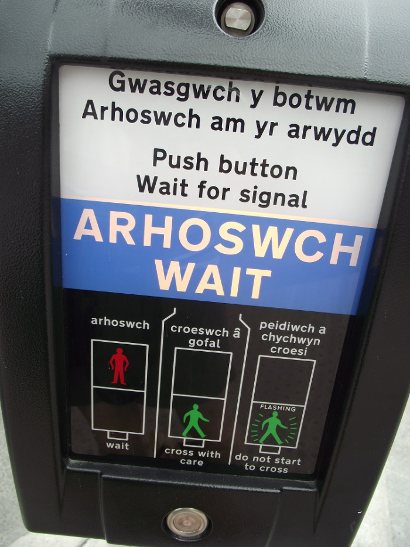
\includegraphics[scale=0.78]{chapters/img/Welsh.png}
        \caption{A zebra-crossing sign in Aberystwyth, Wales, UK (taken by Míša in 2014)}
        \label{fig:Welsh}
\end{wrapfigure}

Limiting ourselves to Britain and Ireland here, although English is about 15 centuries old (\chapref{prehistory}), it is not equally old everywhere. The first English speakers in Ireland that we know of date back to the 12th century; however, it was not until the 16th and the 17th centuries when English\il{English, Irish} was introduced rather more invasively into Ireland with the Plantations\footnote{Plantations refer to instances of confiscation of land in Ireland initiated by the English government. This is one example of colonialism.\is{colonialism}} \citep{Hickey1993}. Today, Irish English is the mother tongue of most inhabitants of the isle of Ireland, with very few native speakers of \ili{Irish} (a Celtic language) left. In a similar way, in Scotland, English\il{English, Scottish} became the official written language in the 18th century, at the point at which Scotland and England had come under the rule of a single parliament and a single monarch \citep[394]{Wells1982b}. Relatively few native speakers of Scottish Gaelic\il{Gaelic, Scottish} -- another Celtic language -- are to be found today (e.g. \citealp{Nance2013}). Finally, the anglicization of Wales took a jump in the 16th century with the Acts of Union \citep{Williams1990}. The \ili{Welsh} language has seen a decline in the number of native speakers; nonetheless, Welsh seems to be the strongest of the Celtic languages spoken in Britain and Ireland today. It is important to mention the Celtic languages in Britain and Ireland here, because they have influenced the respective varieties of English spoken on these isles as we know them today, in different ways (see e.g. \citealp{FilppulaKlemolaPaulasto2008} and \citealp{Hickey2012} as well as \sectref{OE-Celtic} of this book), and the use of these languages is imbued with political significance as well. See Figure \ref{fig:Welsh}, showing Welsh and English.

However, the 20th and the 21st centuries have brought further important factors to consider regarding today's linguistic variation in Britain and Ireland. There are now numerous places in Britain and Ireland with contemporary multicultural, multiethnic, and often multilingual\is{multilingualism} populations.\footnote{See for example the Multilingual Manchester project website: \url{http://mlm.humanities.manchester.ac.uk/}.} Finally, with the political consequences of Brexit playing out at the time of writing, it remains to be seen whether this may have linguistic consequences, such as (further) diversification in English spoken in Northern Ireland and the Republic of Ireland in particular.\il{English, British|)}

\subsection{English in North America}\label{English-NA}\il{English, American|(}
Together with Ireland, Wales, and Scotland, North America can be considered the first colonies\is{colonialism} and dominions of England, with the beginnings of American English ultimately going back to the first settlers in 1607, when Jamestown was founded. The United States of America were also the first to claim their independence in 1776, with a strong sense of national identity,\is{nation-states} which went hand in hand with linguistic national identity as well (more on this is coming in \chapref{LModE}). The Dominion of Canada became self-governing later, in 1867.

The history of American English could certainly not be told without mention of the high degree of language contact, as well as contact between various dialects of English (\chapref{LModE}). To begin with, North America had already been populated by the time English speakers arrived, and its inhabitants -- the Indigenous peoples of the Americas -- spoke a vast array of languages belonging to several language families. Furthermore, English speakers were not the only settlers, nor were they the only incomers.\footnote{As we will see in \chapref{prehistory}, English, \ili{French}, \ili{Russian}, and \ili{Spanish} -- some of the settler-colonial\is{colonialism} languages of the modern period -- all belong to just one language family. On the varieties spoken in North America, often known as \textsc{heritage} languages, see for example the website of the Alliance for the Advancement of Heritage languages here: \url{http://www.cal.org/heritage/}.} Today, the US includes ethnic minorities such as Hispanic and Latino Americans and Asian Americans, as it has throughout its history, and of course the largest ``minority'' is presented by African Americans. Thus, a range of English varieties is to be found in the US (e.g. \citealp{Wells1982c}, \citealp{WolframSchilling-Estes2015}), and more recently researchers have established that there is increasing linguistic diversity in Canadian English\il{English, Canadian} as well, despite the fact that Canadian English is usually considered fairly homogeneous (\citealp{CheshireHardwick1986}, \citealp{Clarke2010}, \citealp{ClarkeElmsYoussef1995}).\il{English, American|)}

\subsection{English in Australia and New Zealand}\label{English-AU-NZ}\il{English, Australian|(}\il{English, New Zealand|(}
The origins of Australian English and New Zealand English go back to 1788 and to 1840, respectively. Note that these two dates refer to times after the American Independence, and at this point a clearly distinct set of varieties of American English (as compared to British English) had already emerged. Australian English and New Zealand English are thus relatively ``young'' varieties of English. Australia became independent in 1901 and New Zealand in 1907. As with all the other varieties of English discussed so far, what would grow into Australian English and New Zealand English did not begin in a linguistic vacuum. To begin with, the first settlers had brought their own dialects, which would later give rise to what we now know as Australian English and New Zealand English (see \chapref{LModE} for more on this). Secondly, Australia and New Zealand were already inhabited by speakers of a range of Australian Aboriginal languages and \ili{Maori}.\footnote{There is an extensive amount of work on the emergence of New Zealand English and the mixing of English dialects brought to a single place by different groups of settlers. See for example the website of The Origins of New Zealand English Project here: \url{https://www.canterbury.ac.nz/nzilbb/research/onze/}.}

Over the years, Australian and New Zealand English have emerged as varieties of English clearly distinguishable from other varieties, although of course similarities also exist, as we will see in the rest of this chapter. Naturally, the presence of languages other than English in both Australia and New Zealand has contributed to the linguistic diversity found in Australian English and New Zealand English (e.g. \citealp{Butcher2008}, \citealp{DArcy2010}, \citealp{Eisikovits1996}, \citealp{Louro2013}).\il{English, Australian|)}\il{English, New Zealand|)}

\subsection{English in India and South Africa}\label{English-I-SA}\il{English, Indian|(}\il{English, South African|(}
One of the reasons to mention Indian English and South African English in this chapter (rather than some other varieties that are equally interesting and important) is that they represent examples of English as an official language introduced as a result of British imperialism,\is{British Empire} without being adopted as the mother tongue by the majority of the population. Thus, the speakers of the local languages have for the most part resisted the shift to English \citep{Mesthrie2015}. Although the British Empire\is{British Empire} was dissolved, together with the examples discussed in §\sectref{English-BI}--\ref{English-AU-NZ}, both Indian English and South African English stand to show that the presence of the Empire has nonetheless had significant effects on the sociolinguistic landscapes of the respective areas.

English was introduced into India in 1602, with the formation of the English East India Company\is{East India Company} (British East India Company). The Company's early activities involved exploitative trading practices, and these subsequently developed into military engagements and outright conquest: see \citet{Dalrymple2019}. India gained independence from the UK fairly recently, in 1947. The beginnings of South African English lie in 1795. South Africa gained its nominal independence in 1910 and full independence in 1931. The downfall of the British Empire\is{British Empire} goes hand in hand with local independence, which is reflected in the linguistic diversity that tends to be more pronounced at such times. In the case of India, we find again that a vast range of languages had been spoken in the region before the arrival of the English language, falling within a number of different language families, e.g. \ili{Austroasiatic}, \ili{Dravidian}, Indo-European (see \chapref{prehistory}), \ili{Munda}, and others. A high degree of language contact of various types has contributed to the variation we find in Indian English (e.g. \citealp{Sailaja2012}, \citealp{Wells1982c}). Turning to South Africa, with a range of Bantu and other indigenous African languages as well as another Indo-European language (\ili{Afrikaans}) present in the region, it is not surprising that South African English represents a variety of English sociolinguistically distinct from other English varieties and involves a range of locally relevant varieties as well (e.g. \citealp{Mesthrie2015} and the references therein).\il{English, Indian|)}\il{English, South African|)}

Standard native Englishes as we know them today once emerged and were further shaped\is{standardization} by contact with languages other than English (more in Chapters \ref{ME}, \ref{OE}, and \ref{prehistory}).


\begin{varietybox}{Language, dialect, or variety?}
How can one tell whether a certain form of language is a dialect or a language in its own right? This is no easy task to resolve. Typically, the decision is made using political rather than linguistic criteria. This would apply to languages such as \ili{Czech} and \ili{Slovak}: Czech and Slovak are mutually intelligible and a Czech and a Slovak can easily communicate without having to learn each other's language. Awareness that the two are separate languages has increased dramatically since the division of the 20th-century state of Czechoslovakia into two countries in 1993. On the other hand, and perhaps more intuitively, languages can show differences in their linguistic structures. Thus, a sentence such as \textit{Dwi'n hedfan yn yr awyr} (\ili{Welsh}), \textit{Létám ve vzduchu} (Czech), and \textit{I'm flying in the air} (English) are sufficiently different for us to conclude that these must be different languages. However, the boundaries are not always so clear. That's because, historically, dialects may develop into distinct languages, so there is a whole cline of possibilities. You'll see more on this in \chapref{prehistory}. Because there are two sets of criteria to use, political criteria and linguistic criteria, but also because the term dialect may be associated with negative connotations in lay use, linguists often resort to the term \emph{variety} instead. This enables us to avoid making (sometimes impossible) decisions and any negative connotations.\is{regional variation|)}
\end{varietybox}

\largerpage
\subsection{Studying variation in contemporary English}
Those of us interested in studying language variation and change\is{language variation and change (field)} in Present Day English are very lucky indeed -- we have linguistic evidence everywhere we turn, in a number of digitalized forms as well as on paper, the former of which encompass platforms as diverse as films, the radio,\is{media} instant messaging logs, discussion forums, podcasts, etc. We can easily analyse English used in a vast array of contexts, which is a luxury we don't have when studying the older periods of the language. It is fairly easy to get very specific types of evidence since there are plenty of users of English around us -- something that cannot be said of, say, English of the 13th century (that is, unless you have the powers of necromancy or time travel). This ease of access to linguistic evidence in Present Day English is very lucky for us indeed. According to the so-called Uniformitarian Principle\is{uniformitarianism} \citep[21--24]{Labov1994}, the linguistic processes observable today should also be assumed to apply in the past, and the other way round. The present can therefore be used to shed light on the past, and vice versa. With more data available for Present Day English and with more advanced technology\is{technology} to record such data, analysing Present Day English can be of great use for understanding the past. 

Present Day English has seen, and continues to see, a great number of changes on all linguistic levels. Some of these changes are locally restricted, as we would expect considering the specific historical contexts of the individual regions\is{regional variation} in which English is used. However, in what follows, we mainly focus on changes that are more global in their nature, occasionally bringing attention to some more local aspects as well.

\section{Sounds}\label{englishtoday-sounds}
Let's first remind ourselves of one of the messages from \chapref{introduction}: letters are not sounds. Because of the fairly widespread standard spelling\is{orthography} (i.e. letters!) and standardized education, looking at how speakers of a range of varieties write is not necessarily the most thrilling thing to do if we're interested in the sounds of Present Day English varieties and how they differ. For that, we'll have to look at how people speak, and that takes us to \glossterm{gl-phoneme}{phonemes} and their phonetic realizations. Let's remember that phonemes are units of sounds that are contrastive. This means that if we replace /t/ with /d/ in English, as in \emph{tick} /tɪk/, we'll get a rather different word (or two words, actually: \emph{Dick} and \emph{dick} /dɪk/). /t/ and /d/ are two phonemes because, if we replace one with the other, this changes the meaning of the word. \glossterm{gl-allophone}{Allophones}, on the other hand, are by definition not contrastive. In some varieties of English, /k/ (just like /t/, and also /p/) can be pre-glottalized\is{pre-glottalization} (e.g. \citealp{Wells1982b}), which means that there is a bit of a sound like that we know from glottalling\is{glottalling} (\textit{butter} [bʌʔə]), except that we also get the [k] sound itself, leading to [tɪʔk]. Whether we pronounce \emph{tick} as [tɪk] or [tɪʔk] does not lead to a change of the meaning of the word.\footnote{Our discussion of allophony is somewhat simplified. If you want to learn more, see Chapter 8 in \citet{DavenportHannahs2013} for more details. If you'd like something advanced about types of phonemic contrasts and allophony, see \citet{Hall2009}.} Allophonic variation is found across all varieties of English.

What's important to realize when it comes to allophones is that we can predict where we find any given allophone. Thus, we can predict that a pre-glottalized\is{pre-glottalization} /k/ or /t/ is not found word-initially (as in \emph{\textbf{c}an}) in the vast majority of English varieties. We can also predict that a pre-glottalized /k/ or /t/ is more likely to occur in the speech of some speakers than others, based on a range of different social factors (e.g. \citealp{Schleef2013}, \citealp{SmithHolmes-Elliott2017}). At some point in the history of English, the plosives /p/, /t/, and /k/ started being pronounced as pre-glottalized.\is{pre-glottalization} This illustrates one of the characteristics of sound change (and most linguistic variation): it is regular.\is{regularity of sound change} This means that any given sound change happens in a particular linguistic context, so all words that happen to contain that context are affected by this sound change.\footnote{Although we do need to note that the role of word-frequency\is{frequency} effects on phonetic variants had been hotly debated since before the field of sociolinguistics was born (see \citealp{Labov1981} for the so-called Neogrammarian Controversy). What we mean by word-frequency effects is, for example, a scenario in which low frequency words (words we don't use particularly often) are less prone to include the new variant, even though they do contain the appropriate environment.} If a variety of English develops pre-glottalization in non-initial /t/, we can fairly safely expect to find a pre-glottalized\is{pre-glottalization} /t/ in \emph{all} words that have a /t/ which is not in a word-initial context (so in words such as \emph{spi\textbf{t}}, \emph{bi\textbf{tt}er} and \emph{pan\textbf{t}}, for instance, but not in words such as \emph{\textbf{T}om}, at least not in most varieties of English).

We will now look in more detail at four sound changes found in Present Day English: glottalling,\is{glottalling} the Northern Cities Shift\is{Northern Cities Shift} (and briefly other similar vowel\is{vowels} shifts), Uptalk or High Rising Terminals (HRTs),\is{High Rising Terminals} and vocal fry or creaky phonation.\is{creaky voice} All of these are regular sound changes in the sense just introduced.\is{regularity of sound change}

\subsection{Glottalling}\is{glottalling|(}
\largerpage
Glottalling has already been mentioned both in \chapref{introduction} and in this chapter. In the glottalling varieties of English, most frequently /t/ (rather than /p/ and /k/) would be realized as a glottal stop of some type ([ʔ]), leading to the words \emph{cup} and \emph{butter} being pronounced as [kʌʔ] and [bʌʔə] rather than [kʌp] and [bʌtə], for example. If you'd like to listen to some examples, use a browser to find e.g. the song P.O.W.A. by M.I.A., and listen to words such as \textit{cut}, \textit{not}, \textit{better}, and \textit{getting}. The specific rules governing when glottalling happens may differ from one variety of English to another (thus demonstrating local tendencies and heterogeneity), but in each variety of English the contexts in which we find glottalling, and the frequency\is{frequency} at which we find it, can be predicted by social factors as well as language-internal, structural factors (see e.g. \citealp{Schleef2013}, \citealp{SmithHolmes-Elliott2017}).

Glottalling is assumed to have started in Edinburgh and, independently of that, also in London, and generally affects /t/ which is not word-initial. No one quite knows when exactly glottalling was introduced into these two varieties of English; however, estimates refer to the latter half of the 19th century (\citealp[208--209]{Beal2004}, and \citealp{Schleef2013} and the reference therein). It seems that the spread of glottalling in Britain took place primarily throughout the 20th century and continues taking place today. Although glottalling is a well-known property of varieties of English spoken in Britain,\il{English, British} recent reports indicate that it is also found in varieties such as American English\il{English, American} \citep{EddingtonTaylor2009} and Australian English\il{English, Australian} \citep[342--3]{CoxPalethorpe2007}, which makes the title of Smith and Holmes-Elliott's paper \citeyearpar{SmithHolmes-Elliott2017}, ``the unstoppable glottal'', rather fitting!\is{glottalling|)}\footnote{And all this despite the fact that the glottal stop has seen plenty of stigmatization during its lifespan: \url{https://tribunemag.co.uk/2020/06/the-glottal-stop}.}

\subsection{Northern Cities Shift (and other shifts)}\label{NC-shifts}\is{regional variation}\is{Northern Cities Shift|(}\is{chain shifts|(}
A complex sound change affecting the vowel\is{vowels|(} system has been reported for the area known as the Inland North\il{English, Inland North} in the US. We will first explain what this sound change involves and then see that, although in some ways it is indeed specific to the Inland North, we also find some interesting parallels in other varieties of English attested in other parts of the world. There are at least two reasons why we should be interested in sound shifts: firstly, they are present in many varieties of English (as well as other languages); secondly, they are a very nice example illustrating the constraints\is{constraints problem} as well as the embedding problems,\is{embedding problem} two of the five essential problems of LVC\is{language variation and change (field)} (see \chapref{introduction}).

The Northern Cities Shift started with the vowel phoneme we find in words such as \emph{cat}. This vowel raised, i.e. it moved upwards in the vocalic space, and started sounding more like an [ɛ $\sim$ eː] rather than [æ] (``$\sim$'' indicates that the quality may vary on a continuum between [ɛ] and [e]). This left space in the vowel system: the phonetic quality of [æ] was no longer ``occupied'' by any phoneme. As it turns out, this was not the case indefinitely, because the quality of the phoneme /ɒ/ (as in the word \emph{lot}) started changing as well, and it started moving to where the original [æ] of ``\textit{cat}'' words was to be found, as shown in Figure \ref{fig:NCS1}.\footnote{See \citet{Nesbitt2018} on some very recent research on ``\textit{cat}''.}

\begin{figure}[H]
    \subfigure[The initial stages of the Northern Cities Shift]{\label{fig:NCS1}
    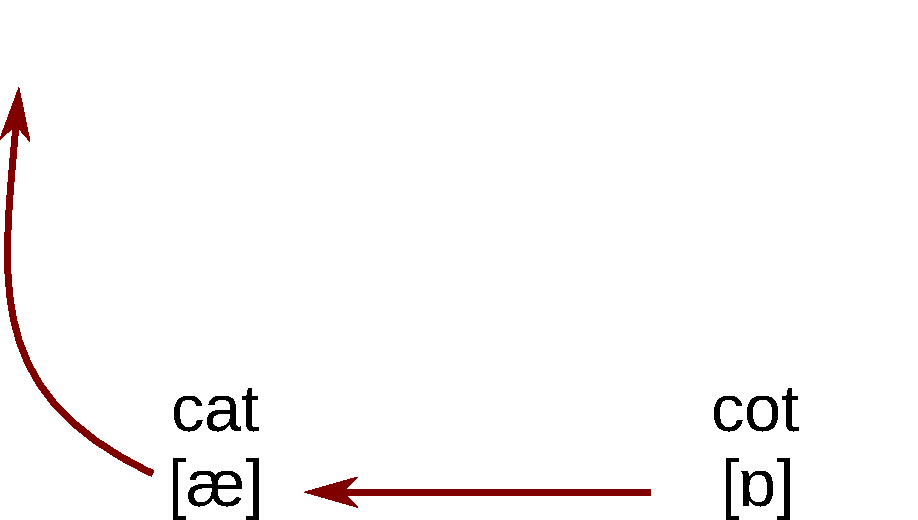
\includegraphics[width=0.45\textwidth]{chapters/img/NCS1a.pdf}
    }
    \subfigure[The Northern Cities Shift]{\label{fig:NCS2}
       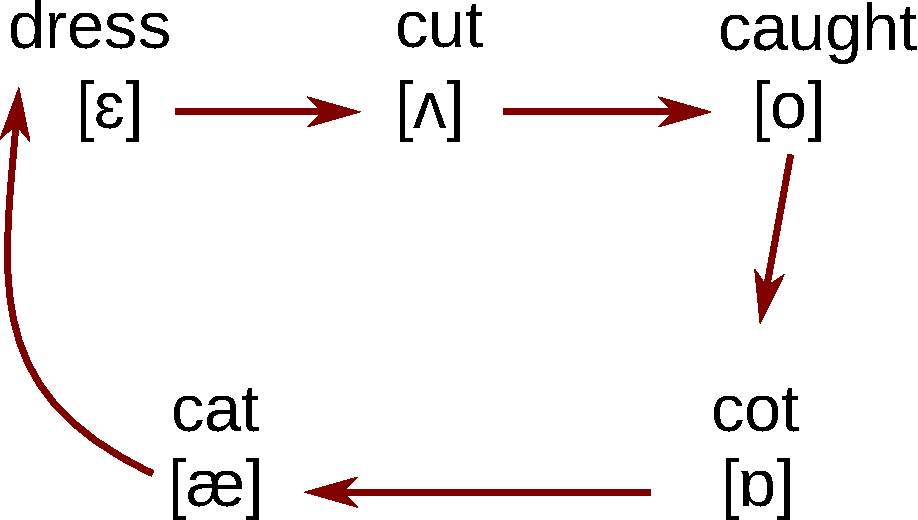
\includegraphics[width=0.45\textwidth]{chapters/img/NCS2a.pdf}
    }
\end{figure}

\noindent Further changes ensued. The vowel in words such as \emph{caught} moved to the vowel space no longer occupied by the \emph{cot} vowel (which had moved to the original \emph{cat} region). This created an ``empty'' area in another part of the vocalic space, and the vowel we find in words such as \emph{cut} /kʌt/ started moving in the direction of the original \emph{caught} vowel. Finally, the vowel in \emph{dress} /dɹɛs/ began moving as well, to the territory left behind by the \emph{cut} vowel (/ʌ/). This leaves us with a situation found in Figure \ref{fig:NCS2}.

You can listen to examples of the post-shift phonetic quality of these phonemes on Eckert's webpage\footnote{\url{https://web.stanford.edu/~eckert/vowels.html}.}; Eckert has investigated the Northern Cities Shift in great detail (e.g. \citealp{Eckert1990}). We can refer to shifts like the Northern Cities Shift as a \textsc{chain shift}, because one change triggers another. It is tempting to ask why a chain shift starts happening in a speech community. One potential explanation proposed for the Northern Cities Shift is that white speakers kept more distance from African American speakers following the African American Great Migration\is{migration} \citep{VanHerk2008}.

The existence of a chain shift of this type is interesting, but what's even more interesting is that the Northern Cities Shift is just one of many shifts that we find across varieties of English. \citet{LabovAshBoberg2006}, for instance, list the Southern Shift, the Pittsburg Shift, and the Back Upglide Shift amongst the main shifts currently taking place in varieties of American English,\il{English, American} in addition to the Northern Cities Shift.\il{English, Inland North} Eckert\footnote{\url{https://web.stanford.edu/~eckert/vowels.html}.} shows a vowel shift in California English,\il{English, California} and reports of shifts are also found for Canadian English\il{English, Canadian} \citep[212]{ClarkeElmsYoussef1995}, New Zealand English\il{English, New Zealand} (e.g. \citealp{Langstrof2006}), and British English\il{English, British} (\citealp{Hickey2018}, \citealp[272--273]{Hejna2015} for Welsh English),\il{English, Welsh} as well as Irish English,\il{English, Irish} Australian English,\il{English, Australian} and South African English\il{English, South African} \citep{Hickey2018}. \citet{Hickey2018} presents an interesting discussion of one specific chain shift (Short Front Vowel Lowering)\is{vowel lowering} which is fairly widespread across the Anglophone world.\footnote{See also \citet{Boberg2019}, who uses the term Short Front Vowel Shift for the same, or at least what seems to be closely related, phenomena.} In the case of these shifts from the 20th and the 21st centuries, it is primarily short vowels that participate in the changes involved.

All these shifts have one thing in common. First, one vowel phoneme undergoes a sound change. Its quality changes, which means that it moves in the vocalic space. What then follows is a change, or movement, of another vowel in the vowel system. And on and on this can go, affecting the phonetic realization of a whole series of vowel phonemes. We start with one vowel changing, and we end up with this one change triggering a whole series of other changes. Hence the name chain shift. But the number of phonemes does not change -- we end up with the same number of phonemes; what changes is the phonetic quality associated with these phonemes. So in the Northern Cities Shift as discussed here, we start with five distinct vowels and we end still with five distinct vowels.

We will see two other fairly famous instances of such chain shifts, one related to vowels (\chapref{EModE}) and one related to consonants\is{consonants} (\chapref{prehistory}), as we continue our journey through the history of the English language.\is{vowels|)}\is{Northern Cities Shift|)}\is{chain shifts|)}

\subsection{Uptalk and High Rising Terminals (HRTs)}\label{HRT}\is{High Rising Terminals|(}
Another innovation that has been spreading throughout the English-speaking world is related to intonation.\footnote{We're very lucky to be able to investigate intonation in Present Day English. This is not something we could really investigate for the older periods of the language.} Uptalk, or High Rising Terminals,\footnote{See \citet[4--7]{Warren2016} for a discussion about the terms Uptalk and HRTs.} refers to the phenomenon in which speakers use a rising intonation (the melody we are familiar with from yes/no-questions) or intonation with a higher pitch, at the end of \textsc{statements}, i.e. in declarative sentences. If you'd like to listen to some examples, visit platforms such as YouTube and search for Uptalk.

Linguists have proposed a range of functions Uptalk performs, amongst which are checking understanding, conveying uncertainty, checking approval, holding the floor, and others \citep{McLemore1991}.

Uptalk is said to have started in California, US,\il{English, Californian} or possibly in New Zealand,\il{English, New Zealand} or Australia\il{English, Australian} (\citealp[37]{Wells2006}, in \citealp{MohamadDeterding2016}). There are nowadays reports of Uptalk in a range of American English\il{English, American} accents (\citealp{McLemore1991}, \citealp{RitchartArvaniti2014}). Since the first reports of Uptalk, researchers have noted the phenomenon in Australian English\il{English, Australian} \citep{FletcherGrabeWarren2005}, British English\il{English, British} (\citealp[36]{Bradford1997}, \citealp{Jespersen2018}, \citealp{ShobbrookHouse2003}), Canadian English\il{English, Canadian} (\citealp{Sando2009}, \citealp{Shokeir2008}), Brunei English\il{English, Brunei} (\citealp{MohamadDeterding2016}), New Zealand English\il{English, New Zealand} (\citealp{Britain1992}, \citealp{FletcherGrabeWarren2005}), and South African English\il{English, South African} (\citealp[146]{Bekker2012}), if not more. While we may think of the rise and spread of Uptalk as a global\is{globalization} change affecting varieties of English, the precise use and forms of Uptalk are nevertheless not the same across these different regions.\is{regional variation} For instance, in her Belfast English\il{English, Belfast} data, \citet[529]{Jespersen2018} observes that Uptalk is used more frequently\is{frequency} by Republicans than by Unionists, signalling political stance in the community. This again shows that global\is{globalization} phenomena can be accompanied with local flavours, presenting us with both a degree of homogeneity and heterogeneity at the same time.

Unlike chain shifts\is{chain shifts} introduced in the previous section (\sectref{NC-shifts}), Uptalk has been negatively stereotyped\is{accentism} in the US in particular, as obvious from the title of the PhD thesis by \citet{Gorelik2016}, which focuses on perception of Uptalk in American English:\il{English, American} \textit{Uptalk as a Powerless Speech Style Characteristic of Job Candidates}. Interestingly, however, \citet{Gorelik2016} did not find that the use of Uptalk would decrease the candidates' employability chances.\is{High Rising Terminals|)}

\subsection{Vocal fry and creaky voice/phonation}\is{creaky voice|(}
The last sound change in progress we will mention is known as vocal fry or creaky voice/phonation. For most speakers, the vocal folds vibrate regularly during much of their speech. When creaky phonation is produced, this is in most cases due to irregular vibration of the vocal folds. The auditory percept is that of a rattling wheel to many listeners. If you would like to listen to some examples, again use platforms such as YouTube and search for vocal fry.

Researchers have been trying to establish the functions of creaky phonation in different varieties. Some of the suggestions that have been brought forward include those that creaky phonation may signal urban-oriented upwardly mobile identity of (accomplished) female speakers \citep{Yuasa2010}, affective stance (see \citealp{Esposito2017} for an analysis of creaky phonation in Lady Gaga's interviews), and a transition of relevance in a conversation \citep{GrivicicNilep2004}.

Creaky phonation has been very negatively stereotyped\is{accentism} in American English,\il{English, American} with creaking individuals being more likely to be associated with various negative attitudes and less likely to be employed \citep{AndersonKlofstadMayewVenkatachalam2014}. Again, as is the case for Uptalk,\is{High Rising Terminals} creaky phonation is not limited just to American English. It has been observed e.g. in Australian English\il{English, Australian} \citep{Sicoli2015}, British English\il{English, British} \citep{Sicoli2015}, and Newfoundland\il{English, Newfoundland} and Labrador English\il{English, Labrador} \citep[154]{Clarke2010}; yet, in these varieties of English, the phenomenon does not seem to carry the same social stigma as in American English.\footnote{\citet{DallastonDocherty2020} recently show that, actually, we know very little about creaky voice in varieties of English -- or even within a single variety of English.}

These aspects all fall within the realm of pragmatics.\is{historical pragmatics} For example, whether someone creaks may indicate that they are about to finish what they say. The functions associated with such linguistic variation go well beyond the level of the sentence. And if someone uses Uptalk,\is{High Rising Terminals} this may imply they are not quite done with what they would like to say. However, as we have discussed above, these phenomena can also be used to provide further information about the speaker's intention or their interpretations of the situational context.

Although we have focused on four sound changes characteristic of Present Day English, there are many more sound changes under way in a range of different accents.\is{creaky voice|)}

\section{Morphology}
\subsection{Absence of -\textit{s}}\label{PDE-s}\is{inflection|(}\is{third person -\emph{s}|(}
Depending on how many and which languages other than English you speak, you may or may not have thought that English does not seem to be particularly rich regarding its \glossterm{gl-inflection}{inflectional} morphology. If we consider the simple present tense, nothing much happens with the verb depending on which person and number the subject\is{subjects} refers to:

\begin{exe}
    \ex I \textbf{like} bumblebees.\is{bumblebees}
    \ex You \textbf{like} bumblebees.
    \ex So we all \textbf{like} bumblebees.
    \ex They \textbf{like} bumblebees too.
    \ex And, surprise surprise, she \textbf{likes} bumblebees as well.\is{bumblebees}
\end{exe}

\noindent The only difference in the verb is found if we contrast the third person singular form with all the other forms: \emph{like} becomes \emph{like\textbf{s}}. In some languages, however, we would get a different verb form in each of these sentences with different grammatical attributes of the subject\is{subjects} (e.g. in \ili{Czech} or \ili{Spanish}), or at least in many more of these sentences. As we will see in the chapters to come, the verbal system of the English language has seen a number of simplifications regarding its inflectional morphology. In fact, some varieties of English show absence of -\emph{s} today even in the 3rd person singular present tense.

The first instances of absence of -\emph{s} date back to the English spoken prior to the colonization\is{colonialism} of North America (at least), and go back primarily to East Anglia and the south of England \citep[102]{Schneider1983}.\is{regional variation} In Present Day English, we find this phenomenon in African American English,\il{English, African American} East Anglia\il{English, East Anglian} \citep{Schneider1983}, Alabama,\il{English, Alabama} Reading,\il{English, Reading} and -- only with the auxiliary\is{auxiliaries} verb \emph{DO} -- in Inner Sydney English\il{English, Inner Sydney} \citep[236--7]{Eisikovits1996}. However, whilst some dialects seem to have unified the verbal \glossterm{gl-paradigm}{paradigm}\is{paradigms} by getting rid of the -\emph{s}, others have generalized the \glossterm{gl-morpheme}{morpheme} across all or more persons and numbers: for instance, \citet[102]{Schneider1983} notes such a tendency for Northern English varieties.\il{English, Northern England}

Although the loss of -\emph{s} may be approached as an instance of the simplification of the system at first, it brings in the potential for new complexities as well. For instance, \citet[27]{MyhillHarris1986} found that in their African American English\il{English, African American} data, the speakers could either use -\emph{s} or leave it out; however, the use of -\emph{s} was associated with narrative clauses whereas its absence was reserved for present-reference contexts. In addition, as we will see in Chapters \ref{LModE}, \ref{EModE}, and \ref{ME}, the loss of verbal endings has been accompanied by the rise of other verbal constructions in the language. We are therefore again observing a phenomenon which presents us with a degree of both linguistic homogeneity and heterogeneity.


\begin{miscbox}{The Northern Subject Rule}  \is{subjects}\is{Northern Subject Rule}
In some English varieties, the use of -\emph{s} is subject to more complex constraints. The best known of these is the \textsc{Northern Subject Rule} of northern British English\il{English, Northern British} varieties.\is{regional variation} Here, the -\emph{s} ending is also used in the third person plural,\is{plurals} as in \textit{The birds\is{birds} sing\textbf{s}}. This only happens when the finite verb occurs right after a subject that isn't a pronoun:\is{pronouns} so, sentences like \textit{The birds often sing} and \textit{They sing} are found alongside \textit{The birds sing\textbf{s}}\is{birds} (see \citealp{DeHaasVanKemenade2014}). What's more, the system is subject to substantial variation, much of it probabilistic. Many varieties around the world have similar, more complex distributions of -\emph{s}: see e.g. \citet{Clarke1997} on Newfoundland English\il{English, Newfoundland} and \citet{Cukor-Avila1997} on African American English.\il{English, African American} The Northern Subject Rule is today considered to be non-standard. Contrary to a common misconception, non-standard forms aren't always (or even normally) recent innovations: very often, non-standard variants are actually much older than their ``standard'' equivalent.\is{standardization} This is the case for the Northern Subject Rule as well: it dates back to Early Middle English \citep{DeHaasVanKemenade2014} and in some form even to Old English \citep{Cole2017}.
\end{miscbox}


\subsection{Verbal concord with collective nouns}\label{Vconc}\is{collective nouns|(}
Collective nouns are nouns such as \emph{cast}, \emph{committee}, \emph{company}, \emph{crowd}, \emph{family}, \emph{government}, \emph{jury}, \emph{staff}, \emph{team}, and names of countries (especially when referring to competing teams). What they all have in common is that they usually involve more than a single individual, hence their name: collective nouns or collectives. In Present Day English, we find a difference in verbal \glossterm{gl-agreement}{concord} (agreement) with regard to collective nouns, primarily between British\il{English, British} and American English.\il{English, American} Where speakers of American English would tend to use a verb in the singular when a collective noun is the subject,\is{subjects} speakers of British English would typically use a verb in the plural,\is{plurals} as shown in the examples below (taken from \citealp[337]{Butters2001}):

\begin{exe}
    \ex 
    Our team wins often. \hfill (American English)
    \ex 
    Our team win/win\textbf{s} often. \hfill (British English)
\end{exe}

\noindent Thus, American English is more likely to exhibit grammatical \glossterm{gl-agreement}{concord}, whereas British English is more likely to show notional \glossterm{gl-agreement}{concord} (based on the semantics of the subject\is{subjects} rather than its morphological number).

Which is older? The British English notional concord option. As \citet{Hundt2003} discusses in her study of the phenomenon, American English of the 20th century is leading in this linguistic change. Other varieties of English tend to show a mixture of these two concord strategies which falls between the state of affairs found in American English and in British English. Some of these varieties include Australian English,\il{English, Australian} New Zealand English,\il{English, New Zealand} Philippine English,\il{English, Philippine} and Singapore English\il{English, Singapore} (see \citealp{Hundt2003} and the references therein): all varieties of English exhibit variable concord to a greater or lesser extent. As \citet[207]{Hundt2003} further notes, there is a trend for the grammatical concord (\emph{Our team wins}) to be gaining in numbers in varieties of English globally. The change from notional to grammatical concord thus leads to more variation found, which illustrates that standard varieties of languages are indeed like the non-standard ones in many ways: they are also subject to change.\is{standardization}\is{inflection|)}\is{collective nouns|)}\is{third person -\emph{s}|)}

\section{Syntax}
In this section, we will look at the rise of a new quotative\is{quotatives} (\emph{BE like}) and the \emph{GET} passive.\is{passive} The former represents a change that many of us may be aware of, whereas the latter seems to be more below our radars.

\subsection{Quotative \emph{BE like}}\label{be-like}\is{quotatives|(}
Quotatives are verbs or constructions that introduce reported speech. Let's have a look at a couple of examples:

\begin{exe}
    \ex And then he \textbf{said}: ``Aren't bumblebees\is{bumblebees} fluffy?''
    \ex He \textbf{sighed}, ``But what about dragonflies? Don't they deserve our attention too?''
    \ex She \textbf{objected}: ``You and your insects. Someone should think of kingfishers too.''
    \ex Ultimately, they all \textbf{cried out}: ``Long live bumblebees,\is{bumblebees} dragonflies, kingfishers, and everyone else.''
\end{exe}

\noindent The verbs in bold all introduce direct speech (marked in what are aptly called quotation marks). Several new quotatives have been recently noticed in English: \emph{BE all}, \emph{GO}, \emph{BE like}, \emph{this is} X (where X stands for the subject whose speech we quote; see \citealp{Buchstaller2001,Buchstaller2013} and \citealp{DArcy2010} for more details). We will only focus on \emph{BE like} here, which we're sure you've all encountered. See for yourself:

\begin{exe}
    \ex She's sitting there and she'\textbf{s like}, ‘Oh my god!'\\
    She'\textbf{s like}, ‘That's your boyfriend?'\\\citep[493]{TagliamonteDArcy2004}
\end{exe}

\noindent The first study of \emph{BE like} focuses on the new quotative in American English\il{English, American} and dates back to 1982 (\citealp{Butters1982}, but see also \citealp{Buchstaller2006}). However, since then it's been reported in an increasing number of varieties of English, at increasing frequencies of occurrence,\is{frequency} including Australian English\il{English, Australian} \citep{Louro2013}, Canadian English\il{English, Canadian} \citep{TagliamonteDArcy2004}, Jamaican English\il{English, Jamaican} \citep{Bogetić2014}, and New Zealand English\il{English, New Zealand} \citep{DArcy2010}.

The attitudes towards this new quotative vary across different varieties. \citet{Buchstaller2006} contrasted attitudes towards \emph{BE like} in American and British English,\il{English, British} and this is what she found. Firstly, the quotative is associated with young speakers in both varieties. However, whilst Americans associate the quotative with California and the Valley Girl, Brits don't. Instead, Brits associate the quotative with speakers whose personality traits are those of giddiness, animatedness, being cool and trendy, being less ambitious, and being less educated. In conclusion, although on the one hand the quotative is spreading across the globe\is{globalization} relatively fast, the connotations associated with it and its socio-pragmatic\is{historical pragmatics} functions are not necessarily the same across the globe. One thing that the new quotative does share across the relevant varieties is that, in a fairly cool way, it's ambiguous as to whether it introduces what the speaker had actually said or just thought, and it may introduce facial gestures as well as direct speech/thought! Thus, for instance, the sentence \textit{George was like ``Aaaaargh!'' for three hours.} does not mean that George literally uttered ``Aaaaargh!'' for three solid hours without pausing for breath. In fact, George may well not have uttered ``Aaaaargh!'' at all -- the new ``quotative'' here can introduce mental states. Perhaps this flexibility may explain why it's been adopted so widely and so rapidly.\is{quotatives|)}

\subsection{\textit{GET} passive}\label{get-passive}\is{passive|(}
The typical example of the \glossterm{gl-passive}{passive} voice in the English language could be something like this:
\begin{exe}
    \ex The hungry bumblebee\is{bumblebees} \textbf{was taken} to the honeysuckle. 
    \ex All my honey \textbf{has been eaten}! 
    \ex Mistakes \textbf{were made}.\footnote{This is a famous example used by a number of politicians, including Jeb Bush.\ia{Bush, Jeb} It has its own Wikipedia page: \url{https://en.wikipedia.org/wiki/Mistakes_were_made}. We are thankful to Sten Vikner\ia{Vikner, Sten} for drawing our attention to this wiki page.}
\end{exe}

\noindent The \emph{GET}-passive is a type of the passive in which the verb \emph{BE} is replaced with the verb \emph{GET}, as in the example that follows, and is found more frequently\is{frequency} in spoken than written language:\footnote{If interested in the formal arguments against all \emph{GET} constructions being suitable examples of \emph{GET}-passives, and whether the term \glossterm{gl-passive}{passive} is always appropriate, see \citet{MitkovskaBužarovska2012}.}

\begin{exe}
    \ex If nothing else, the fans will want to go and see which resident of Springfield \textbf{gets killed} in the last few frames. Could it be Lisa's new Irish boyfriend Colin? After hearing his ghastly singsong ``brogue'', most domestic viewers will wish it so.\\(\citealp[9]{AmadorMoreno2010}, in \citealp[1138]{Nolan2012})
\end{exe}

\noindent The first instances of the \emph{GET}-passive go back to the late 17th century \citep[227]{Fleisher2006}, and the construction started increasing in its frequency\is{frequency} in the latter half of the 19th century \citep[3]{Anderwald2018}, first beginning to attract criticism from prescriptivists\is{prescriptivism} during the 20th century. It has kept on developing a number of more nuanced uses since its inception, throughout Present Day English \citep[1--2]{Anderwald2018}. Anderwald offers interesting sociocultural details that elaborate on why some verbs were more likely than others to be used in this \emph{GET}-construction when it started spreading (such as \textit{to get run over} and \textit{to get mugged}, which refer to activities that one did not necessarily do or arrange oneself in a certain period of time).

The \emph{GET}-passive is a fairly widespread phenomenon, having been studied in British English,\il{English, British} American English \citep{Hundt2001},\il{English, American} Irish English\il{English, Irish} \citep{Nolan2012}, Singapore English,\il{English, Singapore} and Jamaican English\il{English, Jamaican} \citep{Bruckmaier2016}, among others.\is{passive|)}

\section{Lexicon}
\subsection{Global vocabulary}\is{globalization|(}
Due to its geographical spread, English has come into contact with a number of languages, which have introduced many lexical items or new meanings of already existing words into the language. These innovations may be restricted locally, but some may have spread across the globe. Regarding Present Day English, we have for example seen the local differences in the use of the word \emph{café} in Singapore English\il{English, Singapore} and also the \emph{wallah} suffix\is{affixes} used in Indian English\il{English, Indian} (\chapref{introduction}). Other examples are the word \emph{Pakeha} in New Zealand English,\il{English, New Zealand} meaning `stranger, not Maori' and originating in \ili{Maori} (to be precise, Pākehā), where it had the same meaning; \emph{babalaas} `suffering from hangover' in South African English,\il{English, South African} originating in \ili{Afrikaans}; \emph{cwtsh} [kʊtʃ] `a cuddle, cuddly hug, hug' originating in \ili{Welsh}.

However, English has also become important as the language of business communication, aviation, digital technologies,\is{technology} and science,\is{scientific language} which has resulted in the rise of words such as \emph{to google} (first attested in 2000 with an object according to the Oxford English Dictionary),\is{dictionaries} \emph{cursor} (in the sense of a computer mouse cursor first attested in 1967 according to the OED), \emph{to troll} (first attested in the sense of posting hostile messages in online discussions in 1992), \emph{Twitterati} (prolific users of the social network Twitter, first attested in 2006),\is{media} \emph{to photobomb} (to spoil a photo by appearing in it unexpectedly, first attested in 2008), and \emph{to rickroll} (to cause someone to unintentionally watch a pop music video by Rick\is{globalization|)} Astley).\ia{Astley, Rick}\footnote{This term is not yet in the OED, but see \url{https://www.youtube.com/watch?v=DLzxrzFCyOs} for relevant discussion.}

\subsection{Social media, instant messaging, and new expressions}
Some of the technological\is{technology} developments in the 20th and the 21st centuries involve various forms of instant messaging and other digitally-mediated\is{media} communication platforms. \citet{TagliamonteDenis2008} take up and critique the public opinion that instant messaging ruins the English language and is a form of ``bastardization'' \citeyearpar[4]{TagliamonteDenis2008}. Such negative attitudes are, amongst other things, related to the introduction of abbreviated words, such as \emph{lol} (< \emph{laughing out loud}), \emph{btw} (< \emph{by the way}), \emph{omg} (< \emph{oh my god}), \emph{wtf} (< \emph{what the fuck}), etc. However, \citet{TagliamonteDenis2008} show that these new abbreviated lexical items represent a marginal proportion of the vocabulary in their Canadian English\il{English, Canadian} teenage instant messaging data (e.g. 0.02\% of the overall vocabulary in the case of \emph{wtf}, or 0.41\% in the case of \emph{lol}). Thus, the authors conclude that ``[t]he use of abbreviations, short forms, and symbolic uses in IM [Instant Messaging] is without a doubt a new vogue, but much rarer than the media have led us to believe'' \citep[12]{TagliamonteDenis2008}. Furthermore, the fact that we do find such abbreviated lexical items in digitalized communication platforms does not imply these will be used at the same frequency\is{frequency} in spoken English. It's unlikely they are equally frequent in spoken language.\is{frequency}\is{media}

\citet[25]{TagliamonteDenis2008} nonetheless show that ``the variety of English used in the IM corpora\is{corpora} we have studied here is neither a caricature of real language nor some kind of basilectal lowlife'', but rather a new register which could be thought of as a blend of spoken and written language, from the point of view of both structural and lexical similarities and differences (see also \citealp{Baron2008} and \citealp{BiberConrad2019}). That in itself presents a type of language change that doesn't neatly fall within a single linguistic level such as morphology or syntax -- it is indeed a change related to the discourse structure of the language, which may be reflected in the lexicon but also at other levels.

The study of internet\is{media} language has taken off dramatically in recent years -- see \citet{McCulloch2019} for an accessible overview.

\section{Final note}
In our day and age, there are many factors which could no doubt be thought of as leading to homogeneity on various levels of our existence. It's so much easier to travel across the globe,\is{globalization} education is compulsory for much larger portions of the population than used to be the case, and, of course, the means to communicate across distances have been boosted by a number of technological\is{technology} advances (see also \citealp[Chapter 1]{Beal2010}). All these factors are sometimes seen as being the reasons why local varieties of English are dying out (\citealp[Chapter 1, pages 1, 3, and 8 in particular]{Beal2010}). And yet, we have been witnessing many linguistic innovations spreading across different parts of the world and getting utilized and localized by those who adopt them potentially for different purposes in their respective regions.\is{regional variation} But this is not where regional and other linguistic differences stop: any quick browse through an issue of journals such as \textit{Language Variation and Change},\is{language variation and change (field)} \textit{Journal of Sociolinguistics},\is{sociolinguistics} and \textit{English Language and Linguistics} will make it obvious that we're far from a homogeneous English bereft of local features in the 21st century.\is{regional variation}

And now, we encourage you to do the exercises found below. These will enable you to think more carefully about how we can establish whether two varieties of English are more different or more similar. You'll also try to establish which linguistic features are standard and non-standard, or somewhere in between perhaps, and whether you pay equal amount of attention to a range of different types of linguistic variation that surrounds us. And if you do that, then you'll be going home with the take-home messages of this chapter safely sitting in your backpack (or a pocket).

% \label{suggested-exercises}
% \section{Suggested exercises}
\addsec{Suggested exercises}
\begin{exercises}{Practice with varying features}\label{exercise-practice-features}

Look at the sentences below. Which of the variable features discussed in this chapter can you identify? There's one major feature to be identified in each sentence.

\begin{enumerate}
    \item ``My milkshake brings all the boys to the yard\\
    And they're like, it's better than yours'' (\iai{Kelis}, \emph{Milkshake}, 2003)
    \item ``The results will show where your team is on track as well as where problems may be brewing.''\footnote{\url{https://hbr.org/2016/06/the-secrets-of-great-teamwork}, accessed June 2020.}
    \item ``Ahhh The Queen\ia{Windsor, Elizabeth (Queen Elizabeth II)} photo-bombed our selfie!!''\footnote{\url{https://twitter.com/_JaydeTaylor/status/492269017215012864}, 2014, accessed June 2020.}
    \item ``I faked having Covid-19 on Facebook and got arrested''\footnote{\url{https://www.bbc.com/news/technology-52397294}, accessed June 2020.}
    \item ``Pumps and a bump, pumps and a bump\\
    He like the girls with the pumps and a bump\\
    ... one taste and he want it'' (Fifth Harmony, \emph{He Like That}, 2017)
\end{enumerate}
\end{exercises}
\newpage
\largerpage[2]
\begin{exercises}{Tracking words and phrases with Google N-grams}\label{exercise-ngrams}
Use a web browser to visit the Google N-grams site.\footnote{Available at \url{https://books.google.com/ngrams}.} This interface allows you to look at the changing frequency\is{frequency} of words over time in the Google Books \glossterm{gl-corpus}{corpus}\is{corpora} (or short strings of words, called n-grams). You can choose whether to investigate English in general, or American English\il{English, American} or British English\il{English, British} in particular (at the time of writing, other Englishes are sadly not available).

\begin{itemize}
    \item [A.] Look at how frequent the word \textit{fuck} is in the Google Books corpus over time. Go as far back in time as the corpus\is{corpora} allows. 1. Describe the pattern you see. 2. Can you think of any explanations behind this pattern? 3. If you did think of at least one explanation, how could we go about testing whether this may indeed explain what's happening in this specific n-gram?
    \item [B.] Look up \textit{biscuit} and \textit{cookie} and their frequencies across centuries. Go as far back in time as you can. 1. Which one is more frequent? 2. Does the answer depend on the period? 3. Does the answer depend on whether you're limiting your searches just to American or British English? 4. How can we explain the patterns indicated by your searches?
    \item [C.] Think of pairs of words that might overlap in meaning in British and American English, like \textit{biscuit} vs. \textit{cookie} or \textit{tap} vs. \textit{faucet}. Search for these in the British corpus.\is{corpora} What do you see? Can you explain your results?
    \item[D.] In \sectref{be-like}, the quotative\is{quotatives} \textit{BE like} was introduced. Look at the historical trajectory of \textit{BE like}, \textit{SAY}, and \textit{BE all}. Does \textit{BE like} indeed increase as we approach 2020? What happens to the other quotatives? Do you get different results for the British and the American subsections of the corpus?\is{corpora}
    \item[E.] In \sectref{get-passive},\is{passive} the \emph{GET}-passive was introduced. Can you think of a way to investigate the rise of the \emph{GET}-passive\is{passive} using the Google N-gram Viewer? What are the advantages and disadvantages of this method?
    \item[F.] What are the advantages and disadvantages of the Google Books corpus\is{corpora} as a whole?
    \item[G.] Can you think of using Google N-grams in any way either as a researcher or as an English teacher?
\end{itemize}
\end{exercises}

\begin{exercises}{American and British English -- more different or more similar?}\label{AE-and-BE}\il{English, American}\il{English, British}
Are there more differences than similarities between British and American English? Each student/group (as specified by the teacher) should answer the question in a short written piece of no more than 400 words. Feel free to use the extracts in \sectref{text-samples} as well as any other sources that may be of relevance.\\

\noindent\emph{Tips for students}: If you don't know how to begin, you can structure your answer as follows: 1. What is the question? Introduce the question. Don't assume your reader is telepathic.; 2. What do you want to argue for/against?; 3. Show us why you argue the way you do (what's your evidence?); 4. Conclude briefly to remind us of the main argument/point.\\

\noindent\emph{Tip for teachers}: Using group blog entries for this assignment as well as a reasonable deadline is a good idea -- it saves time both for the students and you, and the deadline will allow you to go through the contributions prior to the seminar.\\


\noindent\emph{Tip for teachers}: Add a condition of the students having to use at least one source (or more) to back up their claims, using the reference style of your department.
\end{exercises}

\begin{exercises}{How does English vary?}
\chili{}
Look at the excerpts in \sectref{text-samples}. Can you see any non-standard features?\is{standardization} What linguistic level do they represent? Have you come across them in other varieties of English? What varieties were they? Can you think of any possible reasons why this variation exists?\\

\noindent\emph{Tip for teachers}: Assign different excerpts to different groups of students.
\end{exercises}

\begin{exercises}{Homogeneity vs. heterogeneity}
\chili{}
In Present Day English, do factors such as the advent of digital media,\is{media} generalization of compulsory education, and the increasing ease of travelling opportunities contribute to an increasing similarity, or homogeneity, increasing dissimilarity, or heterogeneity, both, or neither? 

Each student/group (as specified by the teacher) should answer the question in a short written piece of no more than 300 words. Feel free to use the extracts in \sectref{text-samples} as well as any other sources that may be of relevance.\\

\noindent\emph{Tip}: see the tips in exercise \ref{AE-and-BE}.
\end{exercises}

\addsec{Texts}
This section contains texts from different varieties of Present Day English. In this chapter, and in the other chapters, the texts are in reverse chronological order: like the book itself, the selection of texts goes backwards in time.

\begin{texts}{Queen's Christmas Speech}
\label{text-samples}


Below is an extract from the Queen's\ia{Windsor, Elizabeth (Queen Elizabeth II)} Christmas Speech from 2016.\footnote{You can listen to the entirety of it here: \url{https://www.youtube.com/watch?v=ouieLx4VryU}.} The Queen's speech has not escaped the scrutiny of linguists and so we also give you a snippet here.

\begin{quote}
    \internallinenumbers*{}
    Throughout the Commonwealth, there were equally joyful celebrations -- Grenada, the Bahamas, Jamaica, and New Zealand won more medals per head of population than any other countries. Many of this year's winners spoke of being inspired by athletes of previous generations. Inspiration fed their aspiration and, having discovered abilities they scarcely knew they had, these athletes are now inspiring others.
\end{quote}
\end{texts}

\begin{texts}{Kisses don't lie}
\emph{Kisses don't lie} is a song by \iai{Rihanna}, a singer from Barbados, in the Caribbean. The song comes from her 2006 album titled \textit{A Girl Like Me}, and we give you a couple of lines below. Rihanna's song \emph{Work} might be another intriguing example to look up.

\begin{verse}
% \linenumbers*{}
Cause when you kiss me\\
I feel everything that I been missing\\
I try to slow down but my heart won't listen\\
And it's tearing me all up inside\\
And when you touch me\\
I feel a rush but I'm afraid that it might crush me\\
Should I put my trust in something I don't trust in\\
Cause baby kisses don't lie\\
Kisses don't\\
No, they don't\\
Never don't lie.\\
\end{verse}

\end{texts}

\begin{texts}{This is her first publication}\is{poetry}
\emph{This is her first publication} (2004) is a poem by Conor O'Callaghan,\ia{O'Callaghan, Conor} an Irish writer.\footnote{You can access it at the Poetry Foundation at the following link:
\url{https://www.poetryfoundation.org/poetrymagazine/browse?contentId=42229}.}

\end{texts}

\begin{texts}{Excerpt from \emph{The Wire}}
\emph{The Wire} is a crime drama set in Baltimore, which aired between 2002 and 2008. In this extract from the first season (2002), one of the African American characters, D'Angelo, is teaching two others -- Wallace and Bodie -- how to play chess.

\begin{quote}
    \internallinenumbers*{}
    D'ANGELO A'ight, see this? This the king, and he the man.\\ 
    \phantom{D'ANGELO} You get the other dude's king, you got the game.\\
    \phantom{D'ANGELO} But he trying to get your king too. So your gotta protect\\ 
    \phantom{D'ANGELO} it. Now the king move one space in any direction he\\
    \phantom{D'ANGELO} damn please. Like this, and this, and this. But he ain't\is{\emph{ain't}}\\ 
    \phantom{D'ANGELO} got no hustle. So the rest of these motherfuckers\\
    \phantom{D'ANGELO} on the team, they got his back.\\
    \phantom{D'ANGELO} And they run so deep, he ain't\is{\emph{ain't}} gotta do shit.
    
    BODIE\phantom{XXX} Like your uncle.
  
    D'ANGELO Yeah, like my uncle. \emph{[picks up a queen]} You see this?\\ 
    \phantom{D'ANGELO} This the queen; she smart, she fierce.\\ 
    \phantom{D'ANGELO} She move anyway she want as far as she want.\\
    \phantom{D'ANGELO} And she is the go-get-shit-done piece.
  
    WALLACE\phantom{X} Remind me of Stringer.

    D'ANGELO And this over here is the castle, like the stash.\\ 
    \phantom{D'ANGELO} It move like this, or like this.\\
    \phantom{D'ANGELO} \emph{[demonstrates]}

    WALLACE\phantom{X} Yo, stash don't move, man.

    D'ANGELO Come on, yo, think, how many times we move the stash\\
    \phantom{D'ANGELO} house this week. Right? And every time we move the\\ 
    \phantom{D'ANGELO} stash, we gotta move a little muscle with it.

    BODIE\phantom{XXX} True. A'ight, what about them little bald-headed\\
    \phantom{BODIEXXX} bitches?

    D'ANGELO These right here, these are the pawns. They're like the\\
    \phantom{D'ANGELO} soldiers. They move one space forward, only, except\\
    \phantom{D'ANGELO} when they fight, and it's like-\emph{[demonstrates]}-or like this.\\
    \phantom{D'ANGELO} They in the front lines, they be out in the field.
%     \end{linenumbers}
\end{quote}

\end{texts}

\begin{texts}{Tyneside English}\il{English, Tyneside|(}
Britain is full of interesting (and diverse) varieties of English.\is{regional variation} Tyneside English is spoken in the North East of England. Below you get an extract from the Diachronic Electronic \glossterm{gl-corpus}{Corpus}\is{corpora} of Tyneside English (speaker TLSG01, recorded in the 1960s--1970s).\footnote{If you'd like to see more Tyneside English and listen to examples, we recommend the Talk of the Toon webpage: \url{https://research.ncl.ac.uk/decte/toon/}.}

\begin{quote}
    \internallinenumbers*{}
    Speaker 1: ``it's quite nice up here is it''\\
    Speaker 2: ``yes conditions is better''\\
    Speaker 1: ``yes you do you think eh do you find that people around here are fairly neighbourly you know do you know most of the people''\\
    Speaker 2: ``yes they are yes I mean if you were wanting a helping hand they would help you you know''\\
    Speaker 1: ``yes mm-hm''
%     \end{linenumbers}
\end{quote}\il{English, Tyneside|)}
\end{texts}

\begin{furtherreading}
\label{PDE-reading}
As in Chapter 1, \citeauthor{Trudgill1999}'s \citeyearpar{Trudgill1999} paper on standard English and what it is and isn't provides the readers with perspectives on language varieties that happen to be considered standard.\is{standardization}

For good detailed introductions to specific varieties of English, consult \textit{A Handbook of Varieties of English}, edited by Kortmann and Schneider \citeyearpar{KortmannSchneider2004}. The handbook comes in two volumes, one of which focuses on phonetic and phonological aspects and one on morphology and syntax. Wells's three volumes of \textit{Accents of English} are also a very good overview of differences in the sounds of English dialects, i.e. of accent differences: \citet{Wells1982a,Wells1982b,Wells1982c}. There are also two volumes on lesser-known varieties of English: see \citet{Schreieretal2010} and \citet{Williamsetal2015}.

If you are interested in English as a global\is{globalization} language, you may enjoy reading David Crystal's \textit{English as a Global Language} \citeyearpar{Crystal2003b} and Jennifer Jenkins' \textit{Global Englishes: A Resource Book for Students} \citeyearpar{Jenkins2015}. The literature on English in a global context and World Englishes is fairly rich and you will find a lot of reading options.\is{globalization}

Sadly, there's no book that provides an introduction to change in Present Day English. We therefore recommend that you read the individual papers cited in the relevant sections of this chapter if you are really interested in the changes discussed. In addition, \citet{LeechEtal2009} present in-depth research studies of ongoing changes.

General introductions to sociolinguistics are provided by \citet{MesthrieEtal2009} and \citet{Meyerhoff2019}.\is{sociolinguistics}
\end{furtherreading}
